\documentclass[10pt]{article}
\usepackage[utf8]{inputenc}
\usepackage{listings}
\usepackage{float}
\usepackage{graphicx}
\usepackage{fullpage}
\usepackage{caption}
\usepackage{subcaption}
\usepackage{amsmath}
\usepackage{hyperref}
\usepackage{epstopdf}
\usepackage{csvsimple}

%\renewcommand{\thesubsection}{\arabic{subsection}}
\renewcommand{\thesubsubsection}{\alph{subsubsection}}

\title{Pattern Recognition Practical 6}
\author{Group 24: \and Maikel Withagen (s1867733) \and Steven Bosch (s1861948)}
\date{\today}
\lstset{
frame=single, 
numbers=left, 
breaklines=true, 
language=Matlab,
basicstyle=\footnotesize, 
title=\lstname,
showstringspaces=false
}

\DeclareMathOperator*{\argmax}{arg\!\max}

\renewcommand{\thesection}{Assignment \arabic{section}}
\renewcommand{\thesubsection}{\arabic{subsection}}
\begin{document}
\maketitle

\section{}
\subsection{}
The code in section \ref{Ass1} of the appendix was used to acquire the plots given in figure \ref{fig1.1}. As we can see, the sphering changes the signals in such a way that there is no dependency between them anymore.

\subsection{}
The plots show that there is a clear correlation in unsphered signals (they seem to have a linear correlation: for every increase of x, there is an increase in y and vice versa), while the sphered signals do not have such relationships. In the plots of the sphered signals an increase in x does not necessarily lead to an increase or decrease in y (both are possible in either plot).
This is confirmed by the covariance matrices of the sphered signals:
\begin{lstlisting}
>> cov(spheredS(1,:), spheredS(2,:))

ans =

    1.0000    0.0000
    0.0000    1.0000

>> cov(spheredS(3,:), spheredS(4,:))

ans =

    1.0000    0.0000
    0.0000    1.0000
\end{lstlisting}
The covariance matrices are the same as the identity matrices, indicating that there is no dependence between the signal vectors: information about one signal does not give any information about the value of the other and vice versa (the corresponding covariance is 0).

\begin{figure}[H]
  \centering
  \caption{The mixed signals before and after whitening.}
	\begin{subfigure}[b]{.49\textwidth}
		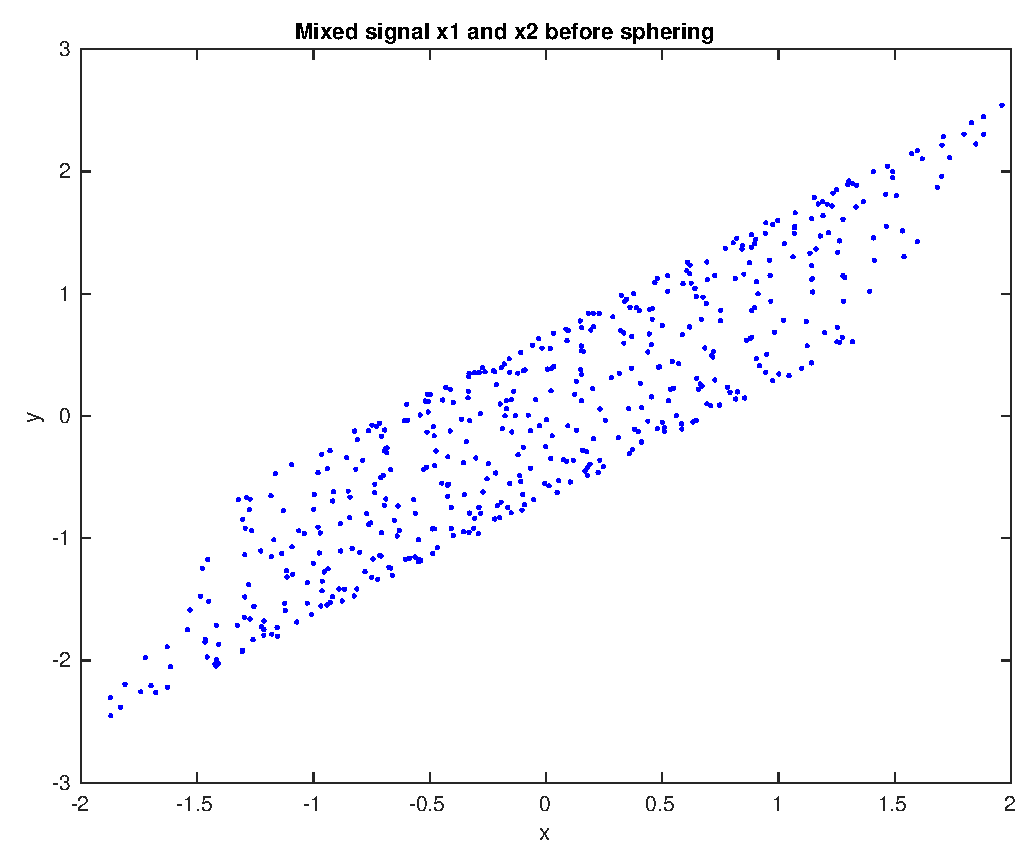
\includegraphics[width=\columnwidth]{Ass1a.eps}
		\caption{}
		\label{fig1a}
	\end{subfigure}  
	\begin{subfigure}[b]{.49\textwidth}
		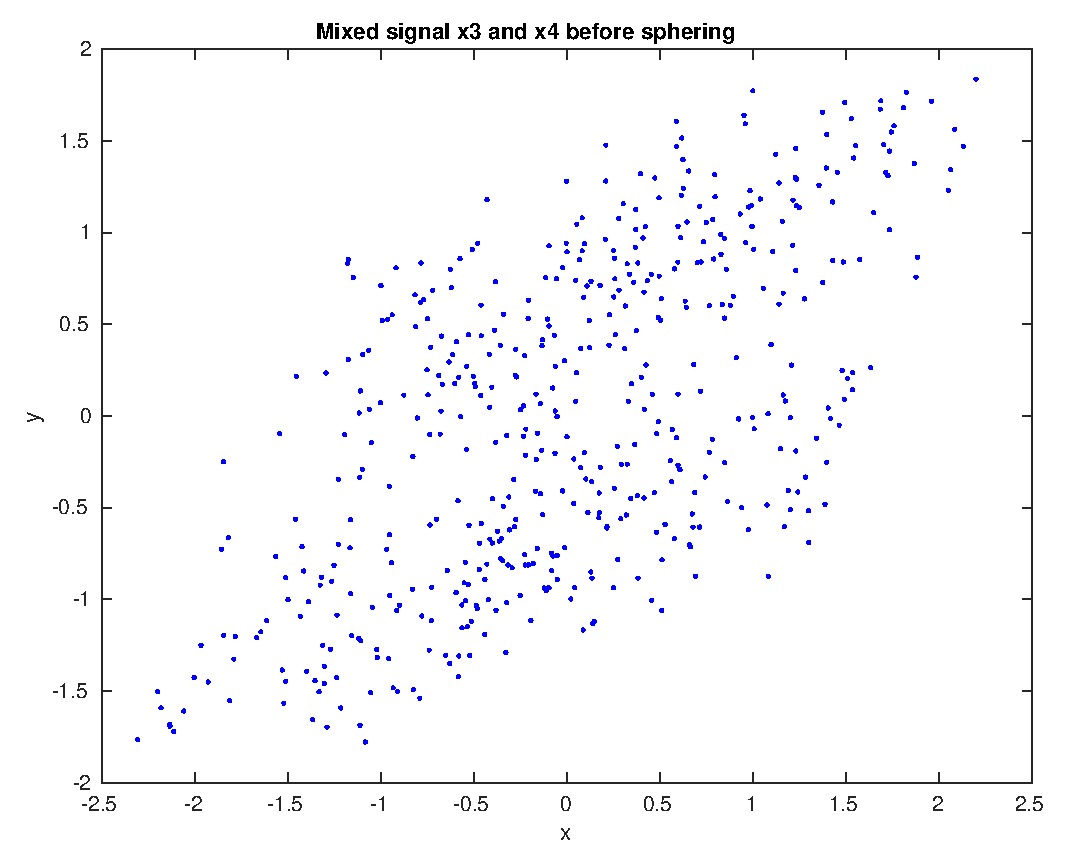
\includegraphics[width=\columnwidth]{Ass1b.eps}
		\caption{}
		\label{fig1b}
	\end{subfigure}
		\begin{subfigure}[b]{.49\textwidth}
		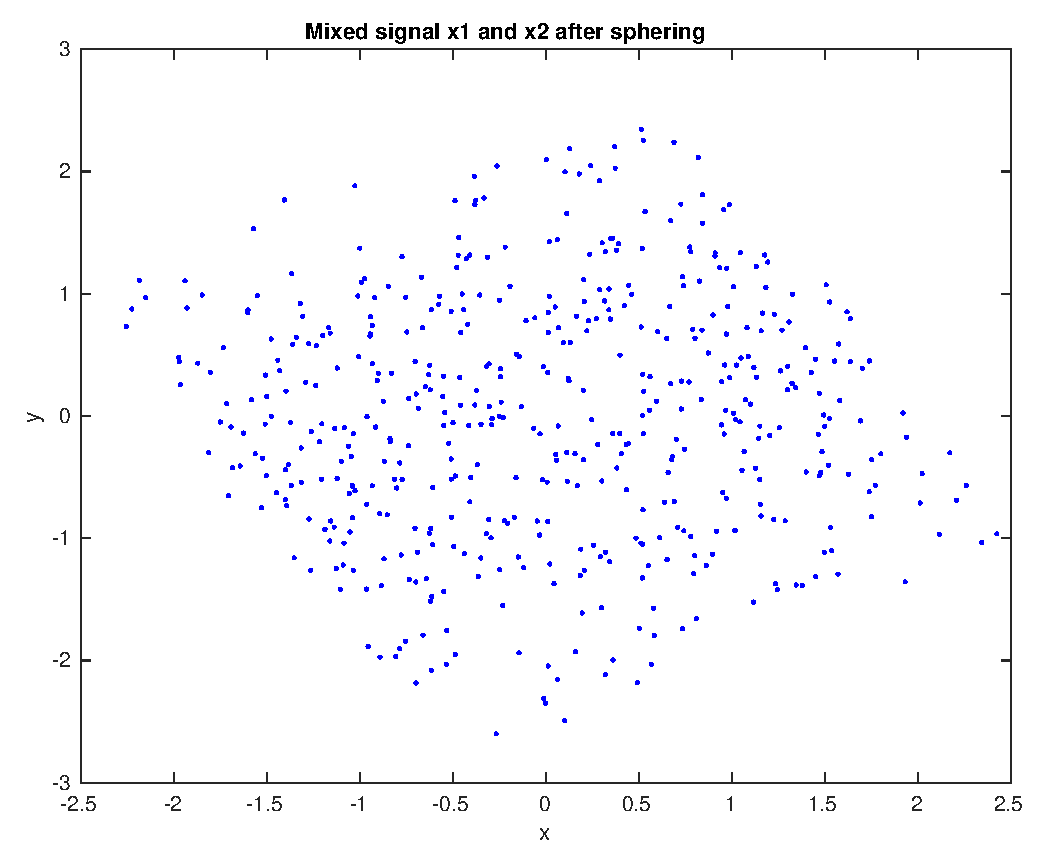
\includegraphics[width=\columnwidth]{Ass1c.eps}
		\caption{}
		\label{fig1c}
	\end{subfigure}  
	\begin{subfigure}[b]{.49\textwidth}
		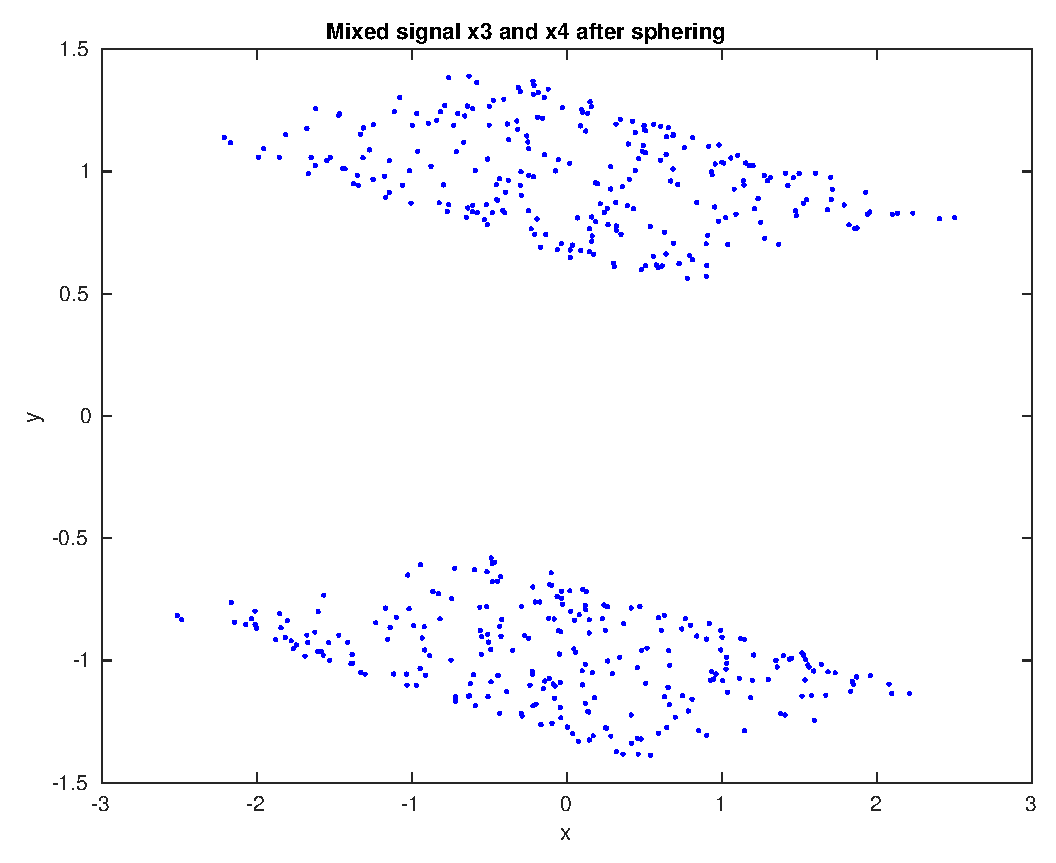
\includegraphics[width=\columnwidth]{Ass1d.eps}
		\caption{}
		\label{fig1d}
	\end{subfigure}
  \label{fig1.1}
\end{figure}

\section{}
Our implementation of the fastICA algorithm with the expansion of assignment 3 is given in section \ref{Ass2} in the appendix (for $n=1$ the code runs for only the first estimated independent component, as is requested in assignment 2).

\subsection{}
The learning rule of fastICA is based on maximizing a measure of non-gaussianity of the input signals. Pre-whitening the data ensures that the used data for the fastICA is statistically independent and maximally non-gaussian, which are assumptions for the fastICA learning mechanism. According to the central limit theorem the mixed signals are more gaussian than the original sources, whitening these mixed signal allows the fastICA to recover the source signals from the mixed ones. 

\subsection{}
The code given in section \ref{Ass2} in the appendix yields the plots given in figure \ref{fig2.1} and \ref{fig2.2} for $numWeight = 1$.
\begin{figure}
  \centering
  \caption{The mixed signals.}
    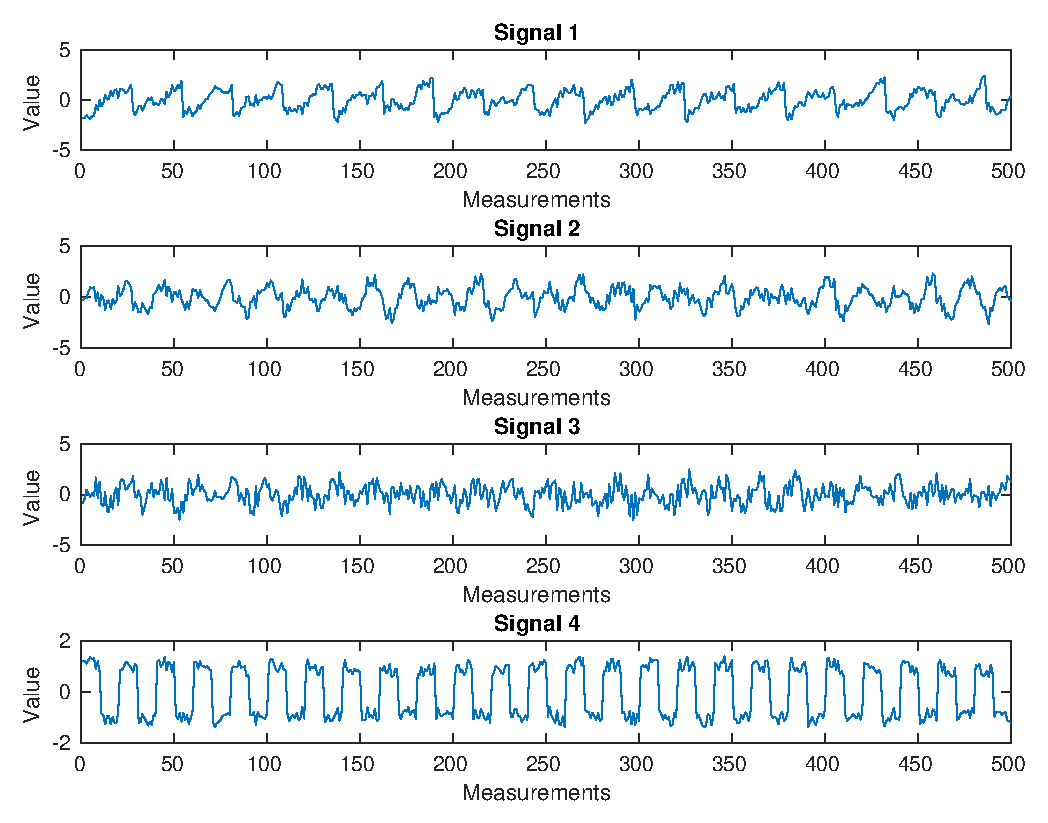
\includegraphics[width=\columnwidth]{Ass3a.eps}
  \label{fig2.1}
\end{figure}
\begin{figure}
  \centering
  \caption{The mixed signals and the estimated independent component ($threshold = 10e-10, numWeight = 1$).}
    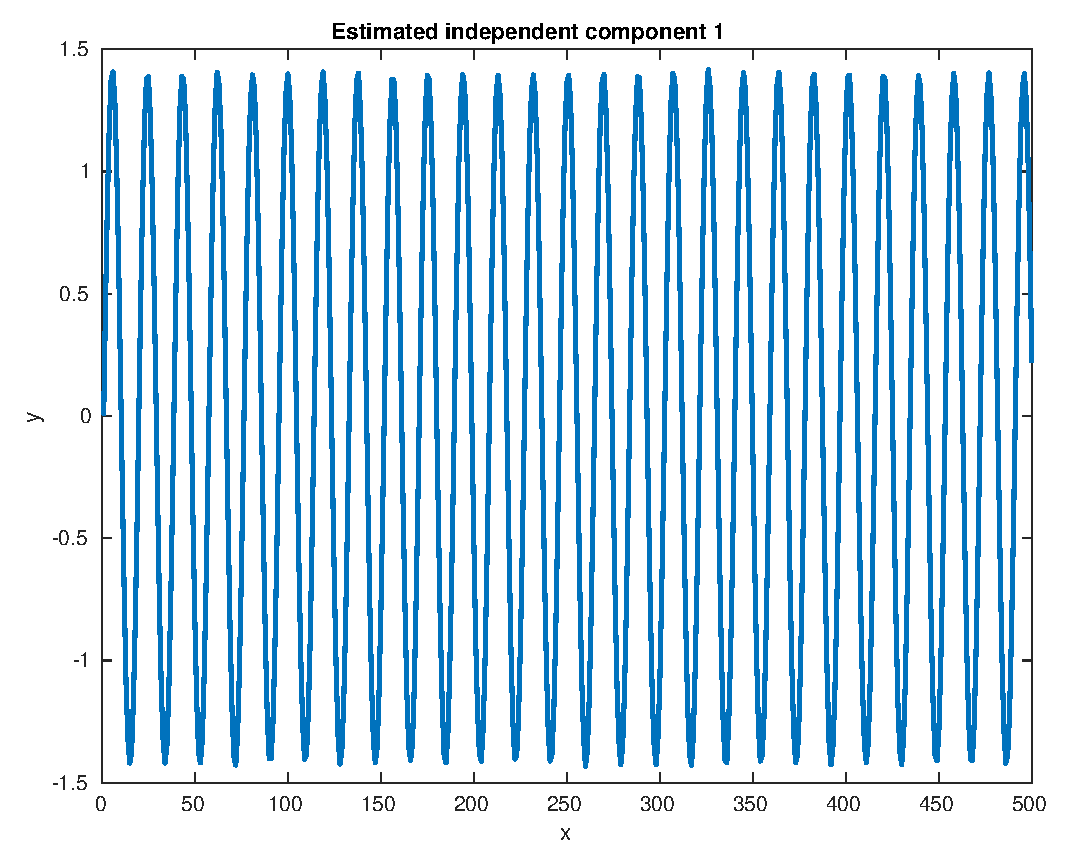
\includegraphics[width=.6\columnwidth]{Ass2b.eps}
  \label{fig2.2}
\end{figure}
Figure \ref{fig2.2} shows that a sinusoid function is the first estimated independent component. When we look at figure \ref{fig2.1} we can see that there is a sinusoid tendency in all four mixed signals, which makes it apparent that a sinusoid function was indeed one of the original source signals.

\section{}
As mentioned above, we used the same code for Assignment 2 and Assignment 3, with a different value for the number of components. We calculated a number of estimated independent components and filtered out the unique ones. We used the decorrelation method mentioned in the slides for week 7 concerning ICA, slide 26.

\subsection{}
The code yields the following conversion matrix:

\begin{lstlisting}
w =

   -0.3317    0.6214    0.4095    0.5798    0.2992   -0.2992
    0.7326    0.3515   -0.4553    0.3640    0.4654   -0.4654
    0.5821   -0.2251    0.7810    0.0226   -0.3989    0.3989
    0.1200    0.6631    0.1227   -0.7286   -0.7313    0.7313
\end{lstlisting}
Every column in this conversion matrix corresponds to a weight vector for one estimated independent component.

\subsection{}
Figure \ref{fig3.2} gives the plots for the six unique estimated independent components (ran with 500 possible components, of which 6 were unique). 

Again we see that the first estimated independent component is a sinusoid function. 
This indicates that there was probably a main sound source that is able to produces sinusoid sounds.
Furthermore, estimated independent components 4-6 all show a sinusoid behavior (sometimes mirrored) similar to estimated independent component 1 (period, amplitude), indicating that they originate from the same source.
Their differences can be explained by noise in the signal.
estimated independent components 2 and 3 show significantly different characteristics from every other component,
indicating they are both coming from a unique sound source.
In conclusion, we can say that there were most likely 3 unique sound sources that have produced the four mixed signals.

\begin{figure}
  \centering
  \caption{The estimated independent components ($threshold = 10e-10, numWeight = 500$ (6 unique)).}
    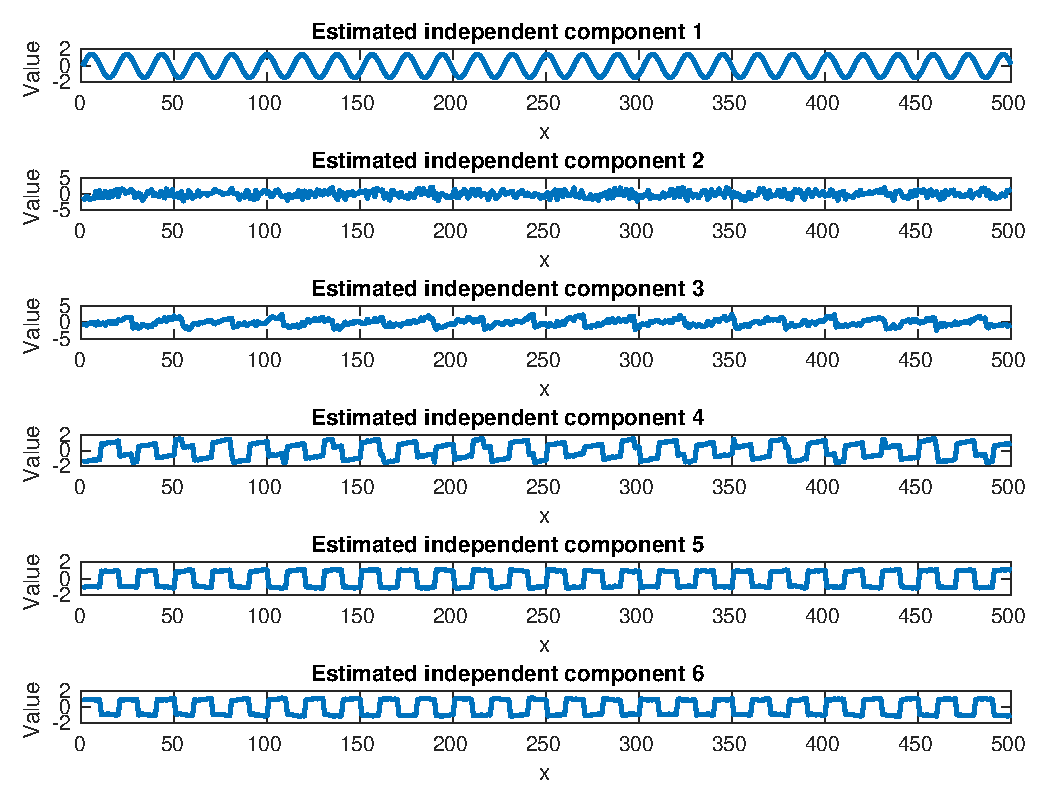
\includegraphics[width=\columnwidth]{Ass3_all.eps}
  \label{fig3.2}
\end{figure}

\subsection{}
The histograms, displayed in Figure~\ref{fig3.3} and Figure~\ref{fig3.4}, confirm that there were at least two unique sound sources. This is shown by the fact that there are two occuring patterns in the histograms.
The histograms for estimated independent componenst 1 and 4-6 show a similar pattern, 
as do the histograms of estimated independent components 2 and 3.
From our results in the previous assignment, we expected to find three distinct patterns in the histograms,
but apparently components 2 and 3 are more similar than we expected.

\begin{figure}
  \centering
  \caption{The estimated independent components ($threshold = 10e-10, numWeight = 500$ (6 unique)).}
    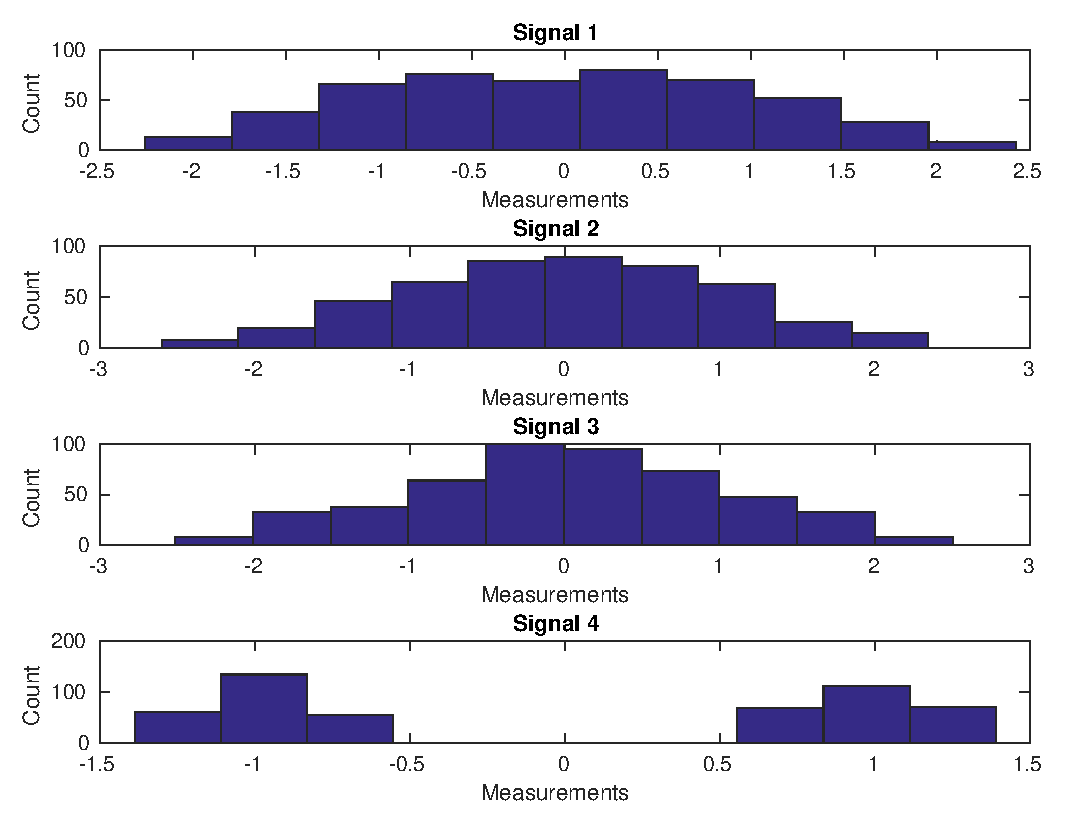
\includegraphics[width=\columnwidth]{Ass3_hist1.eps}
  \label{fig3.3}
\end{figure}
\begin{figure}
  \centering
  \caption{The estimated independent components ($threshold = 10e-10, numWeight = 500$ (6 unique)).}
    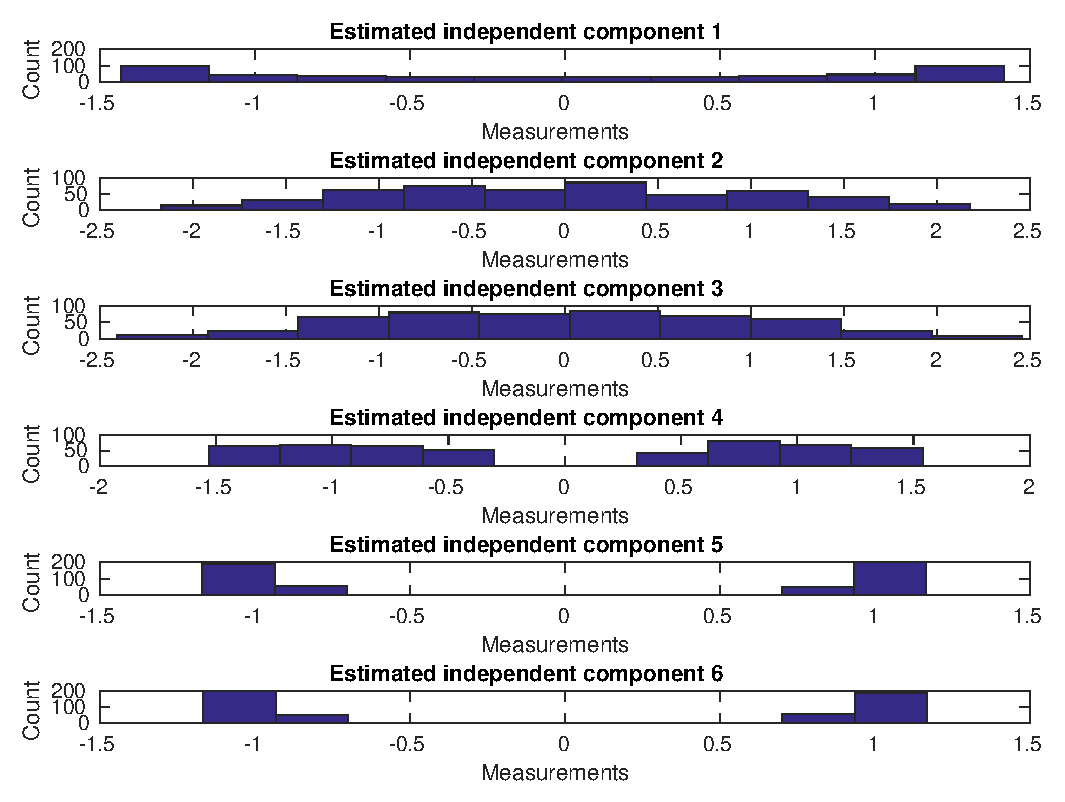
\includegraphics[width=\columnwidth]{Ass3_hist2.eps}
  \label{fig3.4}
\end{figure}


\newpage
\section*{Appendix}
\appendix
\section{Assignment 1}
\lstinputlisting{../Code/Ass1.m}{\label{Ass1}}
\section{Assignment 2 and 3}
\lstinputlisting{../Code/Ass2.m}{\label{Ass2}}

\end{document}
